\section{Maintaining and contributing to a forked repository\label{sec:maintain_repo}}
This section will cover the following points
\begin{enumerate}
	\item Check the status of the forked repository compared to the 'master' repository
	\item Update forked repository
	\item Make changes to your forked repository
\end{enumerate}

\subsection{Checking the status of the forked repository}

To see how your forked repository is compared to the 'master' repository. There is line that is underlined in red shown in Figure~\ref{fig:fork_status}.
	
\begin{figure}[!ht]
	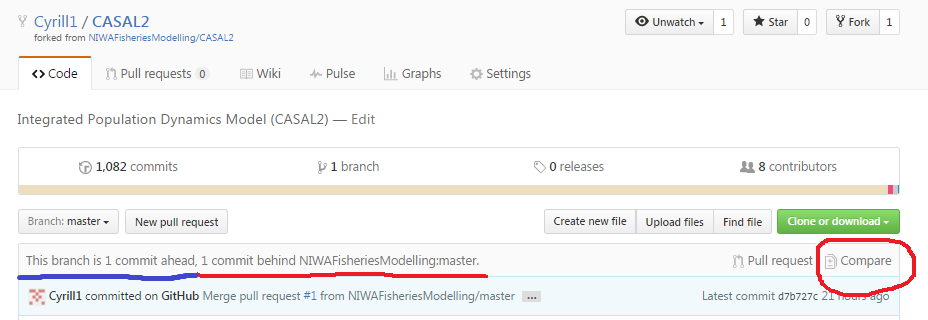
\includegraphics[scale=0.6]{Figures/fork_status.png}
	\caption{Fork status}\label{fig:fork_status}
\end{figure}

This line tells us if we are up to date or as shown in Figure~\ref{fig:fork_status} one commit behind. To update this repository click the 'compare' button which is circled in red. This will bring up a page that will tell you all the changes that have occurred to the 'master' repository. There are two situations that can occur when updating a forked repository. The first and easiest is that there is no conflicts and you can merge teh 'master' changes with ease, the second is there are conflicts.


\subsection{Updating the forked repository}